\section{Lecture 13: Applications of Discrete Time Processing}


\subsection{Introduction}
In the previous lectures in Module 3, we have studied the concepts of sampling of continuous independent variable signals and reconstruction from the sampled signals. In some ways, we thus converted a continuous signal into a discrete one in the process of sampling. Now we wish to apply these concepts learnt to practical scenarios. We motivate this application below.

\subsection{Why Digital Systems over Continuous Systems?}
\subsubsection{Digital vs Discrete Signals}
We first bring out the difference between a digital system and a discrete system. A discrete signal means that the independent variable takes on discrete values rather than continuous values. This we already know. Thus sampling a continuous signal leads to a discrete signal. The result of sampling, a discrete signal, however, takes on arbitrary real values. Implementing this in practice is not possible as we can only represent fixed precision numbers in all our processing devices. Thus, we need to discretise the values taken by the sampled signal i.e. we need to discretise the dependent variable too. The result is then called a digital signal. We give an example below.

%% some image of a sampled and a quantised signal.

\subsubsection{Discrete vs Continuous Signals}
We have already talked about how discrete signals (and digital signals more so) are convenient for processing and and also that they are robust against noise. Somewhat similar is the case with digital and continuous systems. We list below some advantages of digital systems over continuous systems.

\begin{enumerate}
\item \textbf{Flexibility}\\
Digital systems are generally implemented on a digital signal processor (DSP) which, in layman's terms, basically are just computers. The jargon just makes it sound frightening. As is the case with a computer, even a DSP can be made to do a lot of diverse things without much effort. Thus, we just need to change the program and we get a new system implemented without much effort. That however, is not the case with an analog system as it is generally highly specialized and hence restrictive.
\item \textbf{Easy and Low Maintenance}\\
Generally, digital circuit components have a longer life as compared to analog components. Also, a digital system, is by construction more modular as compared to an analog one leading to easy replacement of parts when necessary.
\item \textbf{Generality}\\
Designing an analog system for any given frequency response is often challenging and even practically impossible. This however is not the case with digital systems where we can get as close to the desired response as needed with more processing and possibly more memory.
\end{enumerate}

\subsection{A Digital System}
From the above discussion, it is clear that digital systems are preferred over continuous systems practically. However, the practical world is an analog one and hence the signals there are continuous signals. To use a digital system to process a real world signal, we need to convert the signal into a digital signal, then process it using a DSP and then reconvert it back to an analog signal for it to be of any use to us. This architecture is shown in in figure 1.

\begin{figure}
 	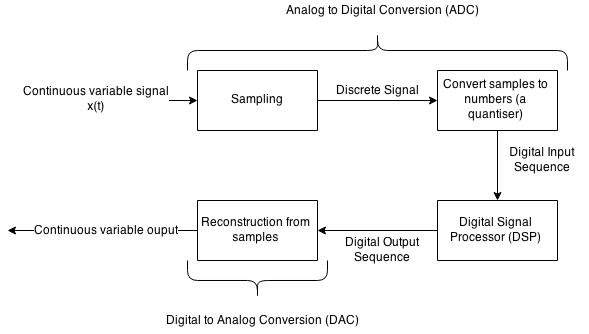
\includegraphics[width=\textwidth]{dsp.jpg}
    \caption{Processing a Continuous Signal Using a DSP}
\end{figure}

As is seen in the figure, we need to sample the input signal (discretise the independent variable) and later quantise it (discretise the dependent variable). Sampling necessitates that the input signal be bandlimited. This is in general not an issue because most of the signals in real life are practically bandlimited given a sufficient frequency range.

\subsection{A Speech Processing System}
We now take a concrete example of a speech signal and discuss the above structure of a digital system in that context.
As we know, a speech signal is generally bandlimited to $4 kHz$. In that case, the Nyquist Sampling Theorem tells us that the signal be sampled at a sampling frequency of more than $8 kHz$. We also, however, know that a margin is better for ease of reconstruction. Thus we decide the sample the speech signal at a frequency of $10 kHz$ i.e. we record 10,000 samples per second. 


\begin{figure}[H]
    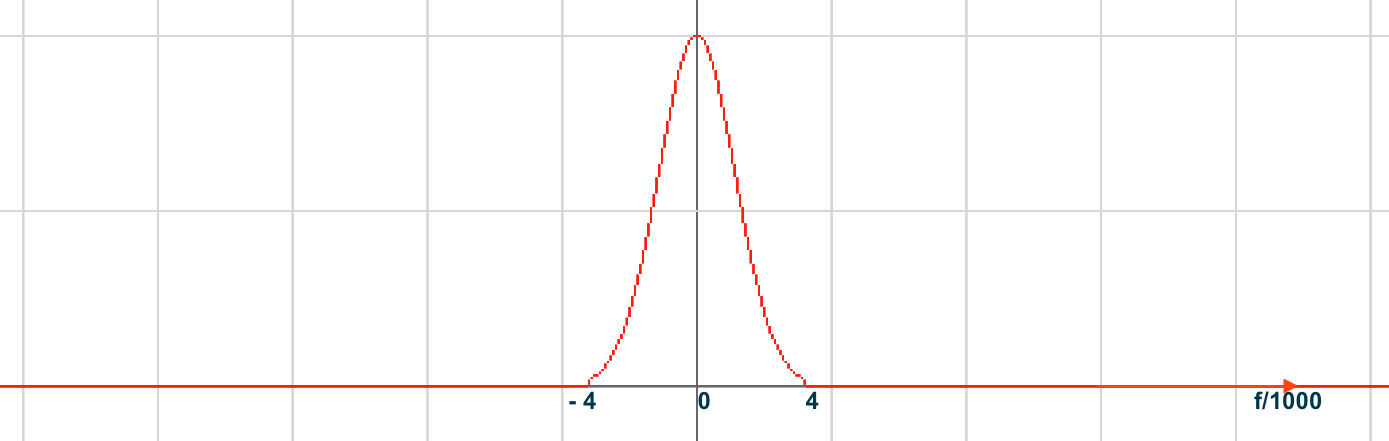
\includegraphics[width=\textwidth]{speech.jpg}
    \caption{Spectrum of a Speech Signal}
\end{figure}%
       

\begin{figure}[H]
    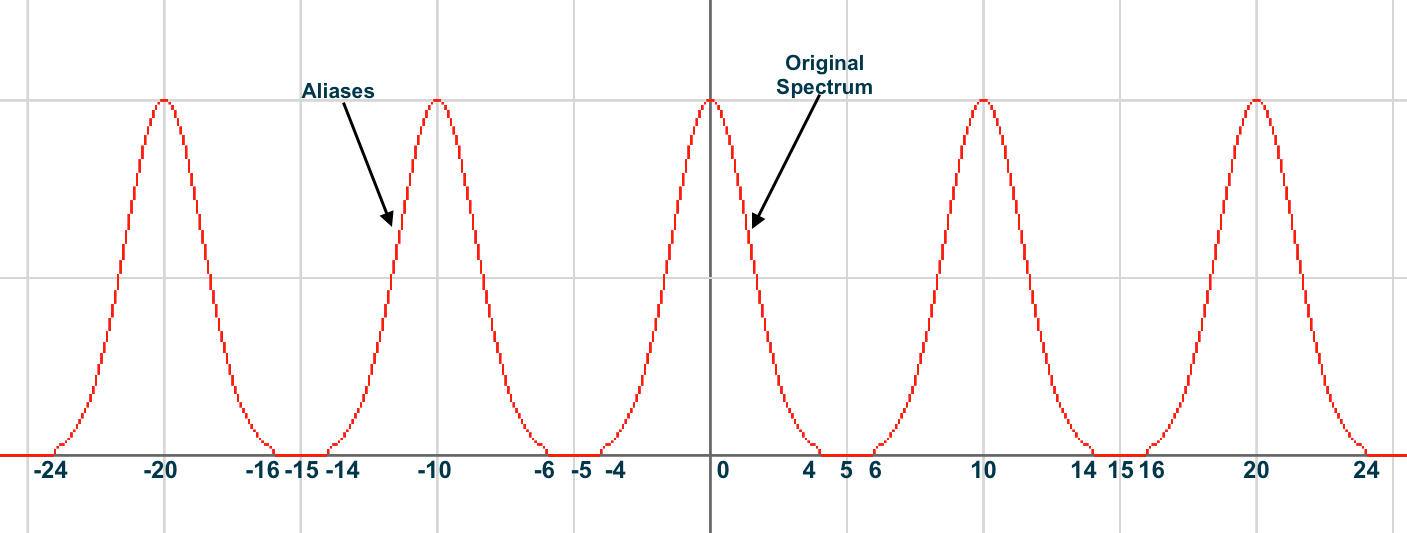
\includegraphics[width=\textwidth]{sampled_speech.jpg}
    \caption{Spectrum of the Sampled Speech Signal}
\end{figure}

Let the frequency spectrum of the speech signal be as shown in figure 2(a) (Note that this is not the spectrum of a real speech signal - which is a lot more complicated - but an illustrative plot) On sampling this signal at $10 kHz$, we get the spectrum shown in figure 2(b). 


\begin{figure}[H]
 	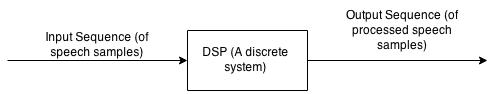
\includegraphics[width=\textwidth]{dig.jpg}
    \caption{A Digital System}
\end{figure}

We then pass these digital samples (which now are just bits) into the digital signal processor to process the signal as desired. %%% What did the DSP do? %%%.
A schematic of this discrete system is shown in figure 4. A discrete system takes as input the input samples and concurrently gives a sequence at the output. After this processing is done, we reconstruct an output signal from the samples from the DSP using a DAC as shown in figure 1.


\subsection{An Overview of a Successive Approximation ADC}
Here we present an overview of a successive approximation analog to to digital converter. A block schematic is given in figure 5. As the name suggests, we start with an approximate binary value of the input voltage and successively (iteratively) improve this approximation. We convert the current approximation of the input (a binary value) into an analog signal with the help of a voltage combiner (this is just a DAC which we look at in the next section). The output of this combiner and the input voltage are then passed to a comparator. Depending on the result of the comparator, we increase or decrease the value of the current approximation (i.e. we improve the approximation in this step). This continues till we can no longer improve the approximation because of the limited precision of the finite number of binary bits available to us.
\begin{figure}[H]
 	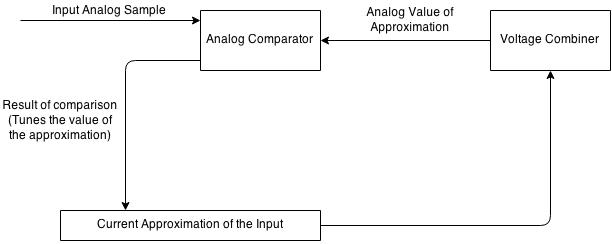
\includegraphics[width=\textwidth]{saadc.jpg}
    \caption{Successive Approximation ADC}
\end{figure}
\subsection{An Overview of a DAC}
Now, we describe a Digital to Analog Converter (DAC). In general, a DAC takes a $n$-bit binary number and converts it into a voltage proportional to the value of the input binary number. We consider the case of a 4-bit DAC as shown in figure 6. $V_{0}$, $V_{1}$, $V_{2}$ and $V_{3}$ are the 4 bits (We assume that the bit $1$ corresponds to a voltage of $5V$ and the bit $0$ corresponds to a voltage of $0V$.). $R_{0}$, $R_{1}$, $R_{2}$, $R_{3}$ and $R_{L}$ are resistors such that $R_{1} = 2R_{0}$, $R_{2} = 4R_{0}$ and $R_{3} = 8R_{0}$. As shown, $I_{0}$, $I_{1}$, $I_{2}$, $I_{3}$ and $I_{L}$ are currents through the resistors $R_{0}$, $R_{1}$, $R_{2}$, $R_{3}$ and $R_{L}$ respectively.
\begin{figure}
 	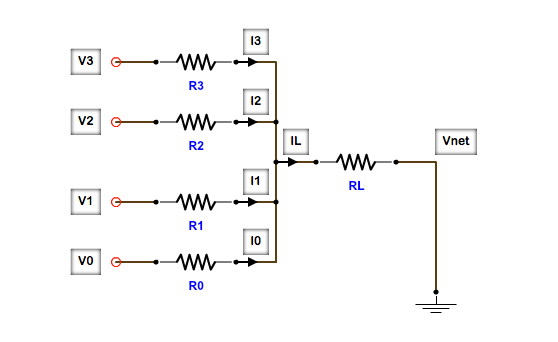
\includegraphics[width=\textwidth]{dac2.jpg}
    \caption{A Possible DAC}
\end{figure}




We have, by Ohm's Law,


\begin{align*}
I_{0} &= \frac{V_{net} - V_{0}}{R_{0}}\\
I_{1} &= \frac{V_{net} - V_{1}}{R_{1}}\\
I_{2} &= \frac{V_{net} - V_{2}}{R_{2}}\\
I_{3} &= \frac{V_{net} - V_{3}}{R_{3}}\\
I_{L} &= \frac{V_{net}}{R_{L}}
\end{align*}



In that case, by Kirchoff's Current Law (KCL), we have, 


\begin{equation*}
	I_{L} = I_{0} + I_{1} + I_{2} + I_{3}
\end{equation*}

Thus,

\begin{align*}
       \frac{V_{net}}{R_{L}} &= \frac{V_{net} - V_{0}}{R_{0}} + \frac{V_{net} - V_{1}}{R_{1}} + \frac{V_{net} - V_{2}}{R_{2}} + \frac{V_{net} - V_{3}}{R_{3}}\\
                             &= \frac{V_{net} - V_{0}}{R_{0}} + \frac{V_{net} - V_{1}}{2R_{0}} + \frac{V_{net} - V_{2}}{4R_{0}} + \frac{V_{net} - V_{3}}{8R_{0}}\\
\end{align*}

Rearranging,

\begin{align*}
	V_{net} (\frac{1}{R_{L}} + \frac{1}{8R_{0}} + \frac{1}{4R_{0}} + \frac{1}{2R_{0}} + \frac{1}{R_{0}}) &=
    \frac{V_{3}}{8R_{0}} + \frac{V_{2}}{4R_{0}} + \frac{V_{1}}{2R_{0}} + \frac{V_{0}}{R_{0}}
\end{align*}

If,

\begin{equation*}
	G_{L1} = (\frac{1}{R_{L}} + \frac{1}{8R_{0}} + \frac{1}{4R_{0}} + \frac{1}{2R_{0}} + \frac{1}{R_{0}})
\end{equation*}

and 

\begin{equation*}
	G_{0} = \frac{1}{R_{0}}
\end{equation*}

Here $G$ stands for conductance, the inverse of resistance. Then we have,

\begin{equation*}
	V_{net} = \frac{G_{0}}{G_{L1}}\frac{1}{8}V_{3} + \frac{G_{0}}{G_{L1}}\frac{1}{4}V_{2} + \frac{G_{0}}{G_{L1}}\frac{1}{2}V_{1} + \frac{G_{0}}{G_{L1}}V_{0}
\end{equation*}


Thus, if $V_{0}$ corresponded to the Most Significant Bit (MSB) of the input binary number and $V_{3}$ corresponded to the Least Significant Bit (LSB), then $V_{net}$ is proportional to the value of the input binary number as is seen. The proportionality constant does not matter a lot because we can always amplify a given voltage if necessary.



\subsection{Frequency Normalisation}
Before we start discussing concrete discrete (or digital) systems, we need get a few boring things out of the way. Notation and convention is one of them. We discuss here something called frequency normalisation. This basically means that we look at quantities all relative to the sampling frequency (or equivalently the sampling interval). Thus, we consider one sampling interval to be a unit length of time. The sampling frequency, which is equal to the reciprocal of the sampling interval (which is now equal to one unit of time) also is equal to unity in these normalised units. Thus, in order to avoid aliasing, according to Nyquist's theorem, the maximum frequency component in the original signal should be less than $0.5$. Similarly, we can also normalise the angular frequency. This will be equal to $2\pi$ times the normalised cycles-per-second frequency. We will use these normalised frequencies in the future lectures to conveniently study more about discrete systems and related concepts.

\subsection*{An example}

Consider a system that takes an input signal as an input and outputs only the positive part of it i.e.,

\[ y(t) = \begin{cases} 
      0 & x(t)\leq 0 \\
      x(t) & x(t) > 0
   \end{cases}
\]


In order to implement this system in the analog domain, we would use a diode. The current-voltage characteristics of a diode (for low values of the voltage) are shown in the figure 8 below.

\begin{figure}[H]
    \centering
    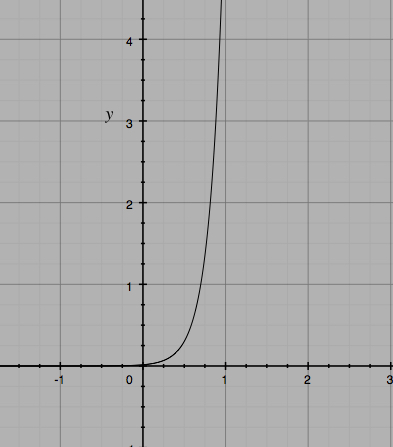
\includegraphics[width=0.5\textwidth]{diode.jpg}
    \caption{A Possible DAC}
\end{figure}

The circuit one would use for this purpose is thus shown in figure 7. 

\begin{figure}[H]
    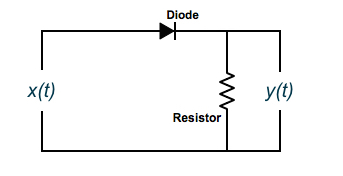
\includegraphics[width=0.8\textwidth]{rec.jpg}
    \caption{A Possible DAC}
\end{figure}

As can be seen from the circuit, the output voltage will be equal to (according to the Shockley diode equation, about which you do not have to know anything :-) )
\[
    y(t) = nV_{T}log(\frac{x(t)}{I_{s}R} + 1)
\]

Here, $n$, $V_{T}$ and $I_{s}$ are some constants characterizing the diode and $R$ is the resistor in the circuit. The point however, is that  the output is not exactly the same as the input when the input is positive and is not exactly zero when the input is negative though it will be close to what is desired. In order to improve the performance, we might want to use better diodes which will lead to a rise in the cost of the system.\\
\indent In the digital domain, however, designing a system to achieve what is desired is both easy and will provide good results if the conversion from the analog to digital domain and back is done properly (which can be done by increasing the sampling rate and decreasing the quantisation interval). Thus, one can see that designing (and improving) a system in the digital domain is much easier than in the analog domain. Also, digital systems provide better results as is seen because unlike analog systems, they are not affected by non idealities of components. (in this case, the diode is non ideal.)




